
%% ============================================================================
%%  It Is Not the Signature: A Discarded Key-Parse Attempt Dominates Token
%%  Validation Cost in a Node.js Service
%%
%%  Submission build for a Springer Nature journal (sn-jnl.cls, sn-basic,
%%  two-column, numeric citations).
%%
%%  EVERY numeric value in the body is a macro from keypath_macros.tex, which
%%  the replication package generates from files under data/runs/ and survey/.
%%  No digit is typed below. keypath_macros_provenance.csv maps each macro to
%%  the file it was read from.
%%
%%  Figures are built from committed CSVs by figures/make_figures.py.
%%
%%  BUILD
%%      latexmk -pdf main.tex          (or: pdflatex, bibtex, pdflatex x2)
%%
%%  If sn-jnl.cls is not installed, this file falls back to `article` plus
%%  sn-fallback.tex so the archive still compiles. See README.md.
%% ============================================================================

\IfFileExists{sn-jnl.cls}{%
  \documentclass[pdflatex,sn-basic,twocolumn]{sn-jnl}%
  \newcommand{\SNJNL}{}%
}{%
  \documentclass[10pt,twocolumn,a4paper]{article}%
}

\IfFileExists{lmodern.sty}{\usepackage{lmodern}}{} % optional; present on Overleaf
\usepackage{amsmath}
\usepackage{amssymb}
\usepackage{graphicx}
\usepackage{booktabs}
\usepackage{url}
\usepackage{xcolor}
\usepackage{listings}

\ifdefined\SNJNL\else%% sn-fallback.tex -- minimal stand-ins for the sn-jnl.cls commands main.tex
%% uses, so the manuscript still compiles under `article` when the Springer
%% class is unavailable. Layout is not the journal's; content is identical.
%% (Stand-in written in the 2026-09-24 revision; replace with your own copy if
%% you have one.)
\usepackage{hyperref}
\makeatletter
\def\title{\@ifnextchar[{\sn@title}{\sn@title[]}}
\def\sn@title[#1]#2{\gdef\@title{#2}}
\newcommand{\fnm}[1]{#1}
\newcommand{\sur}[1]{#1}
\newcommand{\email}[1]{}
\let\sn@author\author
\gdef\sn@authors{}
\renewcommand{\author}{\@ifstar{\sn@auth}{\sn@auth}}
\newcommand{\sn@auth}[2][]{\g@addto@macro\sn@authors{\and #2\textsuperscript{#1}}}
\newcommand{\affil}[2][]{}
\newcommand{\orgdiv}[1]{#1}\newcommand{\orgname}[1]{#1}
\newcommand{\city}[1]{#1}\newcommand{\state}[1]{#1}\newcommand{\country}[1]{#1}
\long\def\abstract#1{\gdef\sn@abstract{#1}}
\newcommand{\keywords}[1]{\gdef\sn@keywords{#1}}
\let\sn@maketitle\maketitle
\renewcommand{\maketitle}{%
  \expandafter\sn@author\expandafter{\sn@authors}%
  \twocolumn[{\sn@maketitle\begin{quote}\small\textbf{Abstract.} \sn@abstract
  \par\medskip\textbf{Keywords:} \sn@keywords\end{quote}\medskip}]}
\newcommand{\backmatter}{}
\newcommand{\bmhead}[1]{\paragraph{#1}}
\makeatother
\fi

\graphicspath{{figures/}}

\input{keypath_macros}

%% ---------------------------------------------------------------------------
%%  A/B corroboration macros (Section~\ref{sec:abcorroboration}).
%%
%%  ALIAS BLOCK — edit ONLY this, then delete it once the names match.
%%  make_keypath_macros.py emits its own A/B names; map them on with \let, e.g.
%%
%%      \let\ABEnabledMean\AbValidationOnMeanUs
%%
%%  or rename in the generator and drop this block. The \providecommand lines
%%  render "??" so an unmapped macro cannot be shipped by accident.
%% ---------------------------------------------------------------------------
\providecommand{\ABRunId}{??}          % run directory, e.g. INSITU-2026-09-14-ab
\providecommand{\ABRate}{??}           % arrival rate, requests/s
\providecommand{\ABWindowSeconds}{??}  % window duration, seconds
\providecommand{\ABEnabledMean}{??}    % per-call mean, validation enabled (us)
\providecommand{\ABDisabledMean}{??}   % per-call mean, validation disabled (us)
\providecommand{\ABEnabledCalls}{??}   % histogram _count delta, enabled
\providecommand{\ABDisabledCalls}{??}  % histogram _count delta, disabled
\providecommand{\ABEnabledLoad}{??}    % 1-min load average at window start
\providecommand{\ABDisabledLoad}{??}   % 1-min load average at window start
\providecommand{\ABDelta}{??}          % enabled minus disabled (us)
\providecommand{\ABDeltaPct}{??}       % delta as a share of the enabled mean
\providecommand{\ABQuantity}{per-request handler time}  % what the means time

%% GUARD. If any A/B macro is still the literal "??", Section 6.4 falls back to
%% a version that reports no numbers, and the build prints a warning. It is
%% therefore impossible to submit a PDF containing "??" in Table 4.
%% Once the alias block above is mapped, this flips itself and the full
%% subsection with Table 4 is typeset. No manual switch to remember.
\newif\ifabdata \abdatatrue
\makeatletter
\newcommand{\ab@unset}{??}  % \newcommand, not \def: both must be \long for \ifx
\newcommand{\ab@check}[1]{\ifx#1\ab@unset\global\abdatafalse\fi}
\ab@check\ABRunId        \ab@check\ABRate          \ab@check\ABWindowSeconds
\ab@check\ABEnabledMean  \ab@check\ABDisabledMean  \ab@check\ABEnabledCalls
\ab@check\ABDisabledCalls\ab@check\ABEnabledLoad   \ab@check\ABDisabledLoad
\ab@check\ABDelta        \ab@check\ABDeltaPct
\ifabdata\else
  \AtBeginDocument{\typeout{^^J*** A/B data not mapped: Section 6.4 is in its
  no-numbers form and Table 4 is omitted. Map the \string\AB... alias block
  to restore it. ***^^J}}
\fi
\makeatother

%% ---------------------------------------------------------------------------
%%  Author-facing placeholders.
%%
%%  Seven facts are known only to the authors and are marked below. While
%%  \showauthornotestrue they are typeset in red so they cannot be missed;
%%  set \showauthornotesfalse for a clean preview. Replace each one and then
%%  delete this block together with the \TODO and \AUTHORNOTE macros.
%% ---------------------------------------------------------------------------
\definecolor{notered}{HTML}{B02A1E}
\newif\ifshowauthornotes
\showauthornotestrue            % <-- set to \showauthornotesfalse to hide

% Inline placeholder: always typesets, highlighted while notes are shown.
\newcommand{\TODO}[1]{\ifshowauthornotes\textcolor{notered}{\textbf{#1}}\else#1\fi}
% Standalone editorial note: vanishes entirely when notes are hidden.
\newcommand{\AUTHORNOTE}[1]{\ifshowauthornotes
  \par\begingroup\color{notered}\footnotesize\noindent
  \textbf{[AUTHORS]\ }#1\par\endgroup\fi}

\newcommand{\LibraryName}{\texttt{jsonwebtoken}}
\newcommand{\LibraryVersion}{\TODO{version~9.0.3}}
\newcommand{\LibraryTag}{\TODO{tag~v9.0.3}}
\newcommand{\CodeFileLines}{\TODO{verify.js, lines 99--110}}
%% CodeFirstLine must be a bare integer (listings uses it arithmetically).
%% The four macros above are produced by make_codepath_figure.py from the
%% pinned release; run it and \input the file it writes, which overrides them:
%%     python3 make_codepath_figure.py path/to/node_modules/jsonwebtoken
%%     \input{figures/codepath_macros}
%% The values below are placeholders taken from the package's master branch and
%% MUST be confirmed against the release you actually measured.
\newcommand{\CodeFirstLine}{99}
\newcommand{\CodeExcerptHash}{sha256:4c4781826f49fa90}
\newcommand{\NaiveFailingTests}{\TODO{both in \texttt{test/wrong\_alg.tests.js}; insert the two \texttt{it()} titles from the failing run}}

%% ---------------------------------------------------------------------------
\lstdefinelanguage{JavaScriptX}{
  keywords={typeof, new, true, false, catch, function, return, null, switch,
            var, if, in, while, do, else, case, break, const, let, try, throw},
  ndkeywords={class, export, import, this, require, module},
  sensitive=true,
  comment=[l]{//},
  morecomment=[s]{/*}{*/},
  morestring=[b]',
  morestring=[b]"
}
\lstset{
  language=JavaScriptX,
  basicstyle=\ttfamily\scriptsize,
  keywordstyle=\bfseries,
  commentstyle=\itshape\color[HTML]{52514E},
  stringstyle=\color[HTML]{1B6E4A},
  numbers=left,
  numberstyle=\tiny\color[HTML]{8A8984},
  numbersep=5pt,
  breaklines=true,
  frame=single,
  rulecolor=\color[HTML]{C9C8C3},
  framesep=4pt,
  columns=fullflexible,
  keepspaces=true,
  showstringspaces=false,
  xleftmargin=2pt,
  aboveskip=4pt,
  belowskip=2pt,
}

\IfFileExists{microtype.sty}{\usepackage{microtype}}{}
\emergencystretch=3em
\hyphenation{
  micro-ser-vices micro-ser-vice micro-bench-mark micro-bench-marks
  cryp-to-graph-ic cryp-tog-ra-phy au-then-ti-ca-tion va-li-da-tion
  in-stru-men-ta-tion con-fig-u-ra-tion im-ple-men-ta-tion
  Ku-ber-netes side-car side-cars name-space through-put
  pre-parsed re-pro-duc-i-ble de-ploy-ment mea-sure-ment
}
\raggedbottom

\begin{document}

\title[It Is Not the Signature]{It Is Not the Signature: A Discarded Key-Parse
Attempt Dominates Token Validation Cost in a Node.js Service}

\author[1,3]{\fnm{Jannatul Ferdous} \sur{Katha}}\email{ferdous.katha@elitelab.ai}
\author[2,3]{\fnm{Tasmia Tahmid} \sur{Prova}}\email{tasmia.prova@elitelab.ai}
\author[3]{\fnm{Md Kishor} \sur{Morol}}\email{kishormorol@ieee.org}
\author*[4]{\fnm{Tze Hui} \sur{Liew}}\email{thliew@mmu.edu.my}
\author[3,5]{\fnm{Dip} \sur{Nandi}}\email{dip.nandi@aiub.edu}

\affil[1]{\orgdiv{Department of CSE}, \orgname{Bangladesh University of Professionals (BUP)}, \city{Dhaka}, \country{Bangladesh}}
\affil[2]{\orgdiv{Department of CSE}, \orgname{Bangladesh University of Business and Technology (BUBT)}, \city{Dhaka}, \country{Bangladesh}}
\affil[3]{\orgname{ELITE Research Lab}, \city{Queens}, \state{NY}, \country{USA}}
\affil[4]{\orgdiv{Faculty of Information Science and Technology}, \orgname{Multimedia University}, \city{Melaka}, \country{Malaysia}}
\affil[5]{\orgdiv{Department of Computer Science}, \orgname{American International University-Bangladesh (AIUB)}, \city{Dhaka}, \country{Bangladesh}}

\abstract{The per-request cost of JSON Web Token validation is routinely
attributed to cryptography. We report that for a widely used Node.js library
the attribution is wrong, and that the natural repair --- moving the cost to key
conversion --- is wrong too. When a shared secret is supplied as a string, which
is what the
library's interface invites --- \LibraryName{} resolves it by attempting to
parse it as an \emph{asymmetric} key first, falling back to the symmetric
constructor only after that attempt throws. The conversion it falls back to
costs \HostCreateSecretKey~$\mu$s and explains nothing. The discarded attempt
preceding it costs \HostProbeThrows~$\mu$s, \HostProbeShareOfCall\% of the call
and its largest single component. Two independent methods agree: differencing
timed conditions across \HostInvocations{} separate processes, and a sampling
profiler attributing a median \ProfHostPct\% of self time to that parse. We do
not separate the cost of the parse attempt from the cost of constructing and
discarding the exception that ends it; the two are reported as one component
and every claim is stated at that granularity. Holding containerisation
constant and varying the runtime, the magnitude co-varies with the bundled
OpenSSL version across four images, spanning \SpanProbeThrows$\times$; two
major engine versions sharing one OpenSSL series do not differ, but the design
cannot separate the faster OpenSSL from the newer engine shipped alongside it,
so we state a co-variation rather than a cause. The cost persists in a deployed
service, measured across seven arrival rates. The avoiding pattern is rare
\emph{in our sample}: \SampleSitesPreparsed{} of \SampleCallSites{} classified
call sites across \SampleRepos{} repositories pass a pre-parsed key, and among
\CounterReposWithVerify{} repositories that both reference the pre-parsing
interface and call the validator, \AdjudicatedGenuineProjects{} use it. These
are samples with unknown inclusion probabilities and no population proportion
follows from them. We propose a fix, and report a constraint on it we consider
the more important result: the discarded attempt is load-bearing for an
existing key-type defence, so the obvious form of the optimisation must not be
applied. All measurements come from one ARM64 host.}

\keywords{JSON Web Token, JWT, key resolution, performance measurement,
benchmarking methodology, Node.js, OpenSSL 3.x, software defect}

\maketitle

%% ============================================================================
\section{Introduction}\label{sec:intro}

Authentication in cloud-native services is commonly described as imposing a
per-request cryptographic cost~\cite{zhu2023dissecting}.
The assumption is old and has been tested before, one layer down: Coarfa et
al.~\cite{coarfa2006performance} instrumented TLS web servers and found RSA
responsible for only a minority of server cost, the remainder falling to
symmetric operations, hashing and protocol handling. Our result is that
argument repeated at the application layer, and reaching a sharper version of
the same conclusion.

The reasoning being tested is intuitive: validating a JSON Web
Token~\cite{rfc7519} means verifying a signature, signatures are cryptography,
and cryptography is expensive relative to parsing. The conclusion usually drawn
is that the cost should be \emph{moved} --- to a sidecar proxy, a gateway, or
dedicated hardware --- because specialised components do cryptographic work
well.

We report that the premise is wrong for the most widely used JavaScript
implementation we could measure. The natural repair is wrong as well. Once the
signature primitive is shown to be a small share of the cost, the remainder is
readily attributed to key material being converted from a string into a key
object on every call. Measuring that conversion directly puts it at
\HostCreateSecretKey~$\mu$s: too small to be the explanation for anything.

The actual mechanism is a control-flow accident, shown in
Figure~\ref{fig:codepath}. Given a secret that is not already a key object, the
library attempts \texttt{createPublicKey()} first and falls back to
\texttt{createSecretKey()} in the exception handler. For an HMAC secret the
first call cannot succeed. Every validation therefore constructs and discards
an OpenSSL parse failure, at \HostProbeThrows~$\mu$s against a total call cost
of \HostJwtString~$\mu$s.

We are careful about what that \HostProbeThrows~$\mu$s is. It is the cost of
the whole discarded attempt: the work OpenSSL performs before deciding the
input is not an asymmetric key, plus the construction and unwinding of the
exception that carries that decision back to the library. We measure the pair.
We do not separate them, and Section~\ref{sec:granularity} states the bound our
data does place on the split. The paper's title and claims are pitched at the
granularity we measured.

\paragraph{Research questions}
\begin{description}
\item[RQ1] Where does the per-request cost of token validation actually go?
\item[RQ2] What does the magnitude of that cost co-vary with?
\item[RQ3] Does it matter in a deployed service, and how common is the pattern
           that avoids it?
\end{description}

\paragraph{Contributions} All supported by measurements in the replication
package~\cite{artifact2026}.

\begin{enumerate}
\item A decomposition of the validation call, by two independent methods,
      locating its dominant component in a discarded key-parse attempt rather
      than in the signature primitive or in key conversion
      (Section~\ref{sec:rq1}).
\item Evidence that the magnitude co-varies with the runtime's bundled OpenSSL
      version rather than with containerisation, together with an explicit
      statement of what the available runtime pairs cannot separate
      (Section~\ref{sec:rq2}).
\item A deployed-service measurement across seven arrival rates, and a survey
      establishing that the avoiding pattern is rare in three samples of public
      code (Section~\ref{sec:rq3}).
\item A fix, and a constraint on it: the discarded attempt is load-bearing for
      an existing key-type defence, so the natural form of the optimisation is
      unsafe (Section~\ref{sec:fix}).
\end{enumerate}

%% ============================================================================
\section{Background and related work}\label{sec:related}

\paragraph{What a validation call does.} A JSON Web Token carries a header, a
payload and a signature over the first two~\cite{rfc7519}. Validating one means
decoding two segments, resolving key material into a form the cryptographic
library accepts, and verifying the signature. The middle step --- key
resolution --- is the subject of this paper, and it is the step most often left
implicit when validation cost is discussed.

\paragraph{Where the cost is usually attributed.} Published measurement of
layered enforcement in microservices concentrates on transport and proxy
layers. Zhu et al.~\cite{zhu2023dissecting} decompose service-mesh sidecar
overhead and show that the dominant contributors depend on configuration and
workload rather than being a fixed tax; we reach an analogous conclusion one
layer up, for application-level validation. Application-level token validation
is itself thinly evidenced, and is commonly reported as a difference between
scenario averages, which attributes to validation every difference between two
runs. We were unable to locate a study that measures the key-resolution step
directly;
we state that as an absence we searched for rather than as a claim about the
whole literature.

\paragraph{Cryptographic cost has been over-attributed before.} Coarfa et
al.~\cite{coarfa2006performance} remains the clearest precedent: measuring TLS
web servers rather than primitives, they found the public-key operation was a
minority of server cost. Work on cryptographic library performance since has
largely stayed at the level of the primitive or the protocol
exchange~\cite{naser2020performance,sikeridis2020assessing}, with Tuveri and
Brumley~\cite{tuveri2019engines} a notable exception in examining how a library
loads and dispatches implementations rather than how fast those
implementations run. Our result concerns neither: it is the cost of getting key
material \emph{into} the library.

\paragraph{Version and environment variation.} That software performance
changes across versions in ways maintainers do not anticipate is established:
Kaltenecker et al.~\cite{kaltenecker2023performance} track performance across
configurable systems' release histories, and Chen and
Shang~\cite{chen2017exploratory} study the code changes that introduce
regressions. Laaber and Leitner~\cite{laaber2018evaluation} assess whether
microbenchmark suites detect such changes at all. Container images make this
concrete by pinning a dependency set implicitly: Cito et
al.~\cite{cito2017empirical} characterise how the ecosystem uses them, and
Malka et al.~\cite{malka2026docker} show that an image tag does not guarantee a
reproducible build. Section~\ref{sec:rq2} is an instance with a measured cost
attached.

\paragraph{Measurement protocol is the thing at stake.} The methodological core
of this paper is not new. Georges et al.~\cite{georges2007statistically}
established that a single execution of a managed-runtime benchmark is not a
measurement, and that intervals must be computed across executions rather than
within one. Mytkowicz et al.~\cite{mytkowicz2009wrong} showed that
environmental details unrelated to the code under study can produce effects
larger than the one being measured, without any obvious mistake. Traini et
al.~\cite{traini2023steady} found that steady state is frequently not reached
at all and that developers misjudge when warmup ends. Our contribution is not
to these methods but is an instance of what they warn about. The attribution
this paper overturns has exactly the structure Mytkowicz et al.\ describe: a
second variable --- the bundled OpenSSL version --- moving unrecorded alongside
the one under study, at a granularity coarse enough to hide it
(Section~\ref{sec:rq2}).

\paragraph{Environment as a confounder.} Laaber et al.~\cite{laaber2019cloud}
quantify how far cloud environments degrade microbenchmark reliability, and
Leitner and Cito~\cite{leitner2016patterns} characterise performance variation
across public infrastructure providers. Their concern is variance between
nominally identical environments. Ours is adjacent and, we think, less
examined: a \emph{systematic} difference between environments that are not
identical and are routinely treated as though they were --- two container base
images differing in a bundled library version.

\paragraph{Cryptographic interfaces are hard to use correctly.} The defect
reported here is not a cryptographic weakness but a consequence of how a
cryptographic interface is invoked, which is a well-documented class. Egele et
al.~\cite{egele2013empirical} found cryptographic misuse widespread in deployed
applications and Georgiev et al.~\cite{georgiev2012dangerous} found certificate
validation broken across a wide range of non-browser software; Nadi et
al.~\cite{nadi2016jumping} attribute much of it to the interfaces themselves
rather than to developer inattention, a position Green and
Smith~\cite{green2016developers} put directly and Indela et
al.~\cite{indela2016helping} respond to with interface proposals; and Acar et
al.~\cite{acar2017comparing} show experimentally that API design materially
changes whether developers produce correct code. Our finding sits within that
line with one difference: the interface here admits a use that is
\emph{correct}, and costly only for a reason invisible at the call site.

\paragraph{Mining public repositories.} Section~\ref{sec:prevalence} draws on
code hosted publicly, and the hazards of doing so are catalogued by
Kalliamvakou et al.~\cite{kalliamvakou2014promises} --- among them that many
repositories are not software projects, that activity is not uniformly
distributed, and that a search result is not a random sample. Our sampling
frame is stated in Section~\ref{sec:frames} with those hazards in view, which
is why no population proportion is computed from it.

\paragraph{The cost of exceptions.} That exceptions are expensive in managed
runtimes, and that their cost is concentrated in construction rather than in
unwinding, is long established: Ogasawara et al.~\cite{ogasawara2006edo}
optimise around exception paths in a Java virtual machine, and Renwick et
al.~\cite{renwick2019lowcost} quantify the cost in a compiled setting.
Parravicini and Mueller~\cite{parravicini2021cost} provide the closest
available cost-attribution baseline for the V8 engine, though on speculation
rather than exceptions. None measures what our result turns on, and
Section~\ref{sec:granularity} states the consequence: we report the parse
attempt and its terminating exception as one quantity because we have no
instrument that separates them.

\paragraph{Key-type confusion.} That a token declaring an HMAC algorithm must
not be validated against asymmetric key material is long established; RFC
8725~\cite{rfc8725} describes the attack and its mitigations.
Section~\ref{sec:fix} reports no new attack. It reports that an existing
defence depends on the control flow whose cost this paper measures, so that
removing the cost naively removes the defence.

\subsection{What we searched for and did not find}\label{sec:gaps}

Five areas bear directly on this result and we were unable to locate verifiable
work in any of them. We state each as an absence we searched for rather than as
a claim about the whole literature; each is also, in part, why the
misattribution corrected here survived as long as it did.

\emph{OpenSSL 3.x performance regressions.} Section~\ref{sec:rq2} reports a
magnitude that co-varies with a bundled OpenSSL version. We found no
peer-reviewed study of performance regressions across the OpenSSL 3.x series.
Evidence exists, but as project issues and mailing-list discussion --- for
instance \texttt{openssl/openssl} issues \#17627 and \#20698, which concern
performance of the 3.x provider and decoder machinery. We cite these as
engineering evidence and note explicitly that they are not peer-reviewed and
were not produced under a measurement protocol we can assess. Consequently
Section~\ref{sec:rq2} reports the co-variation we measured and does not adopt
the mechanism those issues propose.

\emph{Base image to bundled library to application performance.} We found no
academic study tracing that chain. Malka et al.~\cite{malka2026docker} address
build reproducibility and Cito et al.~\cite{cito2017empirical} ecosystem
practice; neither measures how the library version an image pins changes
application performance.

\emph{Cryptographic API misuse as a performance defect.} The misuse literature
cited above treats misuse exclusively as a security problem. We found no work
treating a correct-but-costly use of a cryptographic interface as a latency or
throughput defect, which is precisely what this paper reports.

\emph{Error construction cost in V8 or Node.js.} Our result turns on the cost of
a discarded parse attempt whose terminating exception is a plausible component.
We found no measurement of \texttt{Error} construction cost specific to V8 or
Node.js, so we have no prior baseline to compare against and do not decompose
that cost here. Section~\ref{sec:granularity} states what follows.

\emph{Profiling inside a cryptographic library.} We found no study that profiles
within a cryptographic library to attribute time to key parsing and loading
rather than to the primitive. Section~\ref{sec:rq1} does this from outside the
library, by differencing and by frame attribution, which is weaker than
instrumenting it directly and is the reason Section~\ref{sec:rq2}'s attribution
is stated as a co-variation.

%% ============================================================================
\section{Methodology}\label{sec:method}

\subsection{Unit of measurement}\label{sec:unit}

The unit is one operating-system process, not one call. Each process performs
\HostCallsPerInvocation{} timed iterations of a single condition after a warmup
of half that number, and contributes its median. Reported figures are medians of
per-process medians, with percentile bootstrap intervals taken over processes.

An interval computed over the calls inside one process describes that process's
steady state and is far too narrow: it cannot observe the compilation decisions,
inline-cache states and heap layouts that differ between runs of the same
code~\cite{georges2007statistically}. Conditions in the decomposition of
Section~\ref{sec:rq1} were run in \HostInvocations{} separate processes of
\HostCallsPerInvocation{} calls; conditions in the runtime matrix of
Section~\ref{sec:rq2} in \MatrixInvocations{} processes of
\MatrixCallsPerInvocation{} calls. The largest between-process coefficient of
variation is \HostCvMax\% on the host; in the matrix it is \MatrixCvMax\%,
occurring on the \MatrixCvMaxCondition{} condition under
\MatrixCvMaxEnvironment{} rather than across the matrix generally.

Bootstrap intervals over \HostInvocations{} or \MatrixInvocations{} units are
coarse, and we report them as indicative rather than as calibrated coverage.
Where an interval collapses to a point --- the timer overhead row of
Table~\ref{tab:host} --- it should be read as the clock's resolution showing
through, not as a precise estimate. The per-process values underlying every
interval are in the replication package.

Conditions are interleaved within each round rather than run in blocks. Under
block ordering a thermal excursion or a background process lands entirely on
whichever condition is executing and is indistinguishable from an effect;
interleaved, it is distributed across conditions and appears as between-round
variance. The clock's own cost is measured in the same process as the condition
it accompanies and is reported rather than subtracted: \HostTimerOverhead~$\mu$s
against the smallest quantity reported, \HostCreateSecretKey~$\mu$s.

Differences between conditions are reported throughout as the median of
per-round \emph{paired} differences, not as the difference of two medians. The
two are not identical and the distinction matters at the magnitudes involved;
Section~\ref{sec:residual} and Section~\ref{sec:fix} each rely on it.

\subsection{Decomposing the call}\label{sec:decompose}

\texttt{jwt.verify()} is decomposed into the operations it performs, each timed
in isolation under the same protocol: structural decode; the HMAC primitive with
a string key and with a pre-parsed key; the symmetric key constructor; and the
asymmetric key parse the library attempts first, in both the case where it
throws and the case where it succeeds.

The library measured throughout is \LibraryName{} \LibraryVersion{}, cloned at
\LibraryTag. The code path at issue is shown in Figure~\ref{fig:codepath}.

\begin{figure}[t]
\lstinputlisting[firstnumber=\CodeFirstLine]{figures/codepath_excerpt.js}
\caption{Key resolution in \LibraryName{} \LibraryVersion{},
\texttt{\CodeFileLines}. Verbatim but for the common leading indentation,
which is removed to fit the column; line numbers are the file's own. A secret
that is not already a \texttt{KeyObject} is offered to
\texttt{createPublicKey()} first, and \texttt{createSecretKey()} is reached only
from the exception handler. For an HMAC secret supplied as a string the outer
\texttt{try} can never succeed, so the asymmetric parse is attempted and
discarded on every validation. The excerpt is extracted from the pinned release
by \texttt{analysis/make\_codepath\_figure.py} and pinned by content hash
\texttt{\CodeExcerptHash} in the replication package~\cite{artifact2026}.}
\label{fig:codepath}
\end{figure}

\subsection{Separating the runtime from the deployment}\label{sec:matrix-method}

A host microbenchmark compared against an in-container measurement cannot
support an attribution to deployment: those two environments differ in more than
deployment, and any of the differences could carry the effect. Here
containerisation is held constant and the runtime is varied instead:
four container images spanning two OpenSSL series and three V8 major versions,
on one machine under one container engine.

The pair carrying most of the inference is Node \NodeEighteenNodeMajor{} and
Node \NodeTwentyNodeMajor: they ship V8 \NodeEighteenVeight{} and V8
\NodeTwentyVeight{} respectively while sharing the OpenSSL
\NodeEighteenOpensslSeries{} series. In stock images Node and OpenSSL versions
otherwise co-vary, which would leave the attribution underdetermined. Because
that pairing carries the attribution, the runtime identity of each image ---
Node, OpenSSL and V8 version, libc, architecture and image digest --- is
recorded as a datum and cross-checked against the versions each measurement row
carried. That check found \IdentityMismatches{} mismatches across the matrix.
Section~\ref{sec:cannot-separate} states what this design still cannot separate.

\subsection{In-situ measurement}\label{sec:insitu-method}

The deployed service exposes a histogram timing the verification call alone. The
instrument is a \emph{paired-scrape difference}: the cumulative histogram is read
before and after each arrival-rate step, and the two readings are differenced,
which isolates that step's distribution from the cumulative counters. Means are
computed as the difference of the histogram's \texttt{\_sum} divided by the
difference of its \texttt{\_count}, so they are exact and do not depend on bucket
boundaries; bucket resolution bounds the reported percentiles only.

Seven arrival rates are driven, and the whole sweep is run twice on one process:
once in ascending order and once in descending order. We report the \emph{range
across the two passes}. This is a range of two, not a confidence interval; no
standard error is computed from it, and it is not written as a symmetric
tolerance. The opposite-order design also serves as a drift test, which
Section~\ref{sec:drift} reports.

One process and two passes is the whole of the in-situ evidence. It is sufficient
to establish that the cost is present in deployment and of what order; it is not
sufficient to characterise the shape of the cost-versus-rate relation, and
Section~\ref{sec:insitu} is written accordingly.

\subsection{Prevalence: three instruments, three frames}\label{sec:frames}

Prevalence is approached with three instruments that fail in different ways.
Their sampling frames differ and are not interchangeable, so no population
proportion is computed from them. All three were captured on \PopCapturedAt.

\emph{Population co-occurrence counts.} Code-search counts over public
repositories, in four cells: two languages by two import forms. The denominator
of a cell is files importing the library; the numerator is files that \emph{also
mention} the pre-parsing interface. This measures co-occurrence of two strings in
one file, not verified usage. The denominators are returned rounded --- each is
an exact multiple of $1024$ --- so they are magnitudes rather than counts
established file by file.

\emph{A classified sample of call sites.} Call sites located by search,
deduplicated to one file per repository so that no project dominates, with the
key argument traced within its file. This is a convenience sample from a
relevance-ranked, undocumented ranking; inclusion probabilities are unknown and
no weighting back to the population is possible.

\emph{A targeted counter-search.} Every file co-occurring the library with the
pre-parsing interface, fetched in full and adjudicated by hand. This frame is
deliberately biased toward finding the pattern --- that is its purpose as a
negative control --- and it is therefore disqualified as a prevalence estimator.

Three reasons preclude a population-level prevalence. The population numerator
and the verified numerator measure different things: of \AdjudicatedTotal{}
automatically flagged call sites, \AdjudicatedFalsePositive{} were false
positives on hand inspection, so the co-occurrence signal carries an error rate
that would be inherited, unmeasured, by any extrapolation. The sample has no
inclusion probabilities. And the counter-search is selected on the outcome.
Results are therefore reported \emph{in our sample}, or \emph{among repositories
that co-occur the interface and call the validator}, and never as a population
proportion. This constraint is carried into the abstract and the conclusion.

\subsection{Host state is recorded per measurement}\label{sec:hoststate}

A service measured on a host it shares with its own load generator, ingress and
sidecars is measured together with whatever else that host is doing. We observed
this directly while building the instrument: re-running one configuration with a
background indexing process consuming host CPU moved the point at which
throughput collapsed by hundreds of requests per second, and both runs are
committed in the replication package~\cite{artifact2026}. A curve that moves
with unrelated host activity does not characterise the service, and this paper
therefore makes no capacity claim. Every in-situ window instead carries the host
load average observed during it, committed beside the measurement, and
Section~\ref{sec:load} uses it.

%% ============================================================================
\section{RQ1: Where the cost goes}\label{sec:rq1}

\subsection{The decomposition}

Table~\ref{tab:host} gives each operation in the validation path, timed in
isolation on the host under the protocol of Section~\ref{sec:method}, and
Figure~\ref{fig:decomposition} plots it.

\begin{table}[t]
\caption{Cost of each operation in the validation path. Medians of per-process
medians over \HostInvocations{} processes of \HostCallsPerInvocation{} calls;
95\% percentile bootstrap intervals over processes, which with
\HostInvocations{} units are indicative rather than calibrated
(Section~\ref{sec:unit}).}
\label{tab:host}
\small\setlength{\tabcolsep}{4pt}
\begin{tabular}{@{}lrr@{}}
\toprule
Operation & Median & 95\% interval \\
           & ($\mu$s) & ($\mu$s) \\
\midrule
\texttt{verify()}, string secret   & \HostJwtString      & [\HostJwtStringCiLo, \HostJwtStringCiHi] \\
\textbf{discarded asym.\ parse}    & \textbf{\HostProbeThrows} & [\HostProbeThrowsCiLo, \HostProbeThrowsCiHi] \\
successful asym.\ parse            & \HostProbeSucceeds  & [\HostProbeSucceedsCiLo, \HostProbeSucceedsCiHi] \\
\texttt{verify()}, pre-parsed key  & \HostJwtPreparsed   & [\HostJwtPreparsedCiLo, \HostJwtPreparsedCiHi] \\
HMAC, string key                   & \HostHmacString     & [\HostHmacStringCiLo, \HostHmacStringCiHi] \\
HMAC, pre-parsed key               & \HostHmacKeyObject  & [\HostHmacKeyObjectCiLo, \HostHmacKeyObjectCiHi] \\
structural decode                  & \HostDecodeOnly     & [\HostDecodeOnlyCiLo, \HostDecodeOnlyCiHi] \\
\textbf{symmetric key constructor} & \textbf{\HostCreateSecretKey} & [\HostCreateSecretKeyCiLo, \HostCreateSecretKeyCiHi] \\
timer overhead                     & \HostTimerOverhead  & [\HostTimerOverheadCiLo, \HostTimerOverheadCiHi] \\
\bottomrule
\end{tabular}
\end{table}

\begin{figure*}[t]
\centering
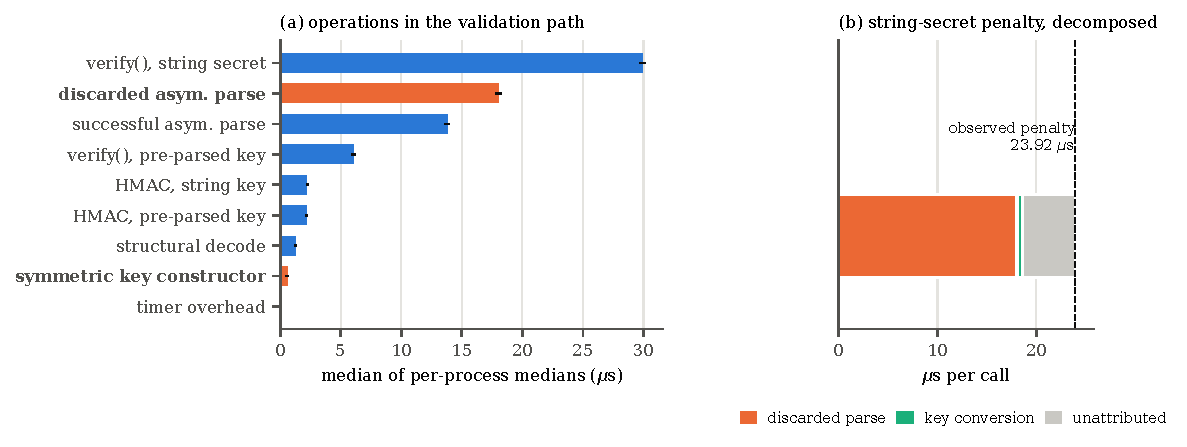
\includegraphics[width=\textwidth]{fig_decomposition.pdf}
\caption{(a) Every operation in Table~\ref{tab:host}, on a linear scale, with
the two components the paper turns on emphasised; whiskers are the 95\%
percentile bootstrap intervals over \HostInvocations{} processes. (b) The
\HostStringPenalty~$\mu$s penalty for supplying a string secret rather than a
pre-parsed key, decomposed. The three segments are medians of per-round paired
differences, not a partition of a single measurement, and they do not sum to the
penalty: the \DecompResidual~$\mu$s remainder is unattributed
(Section~\ref{sec:residual}). Both panels are generated from
\texttt{figures/data/} by \texttt{figures/make\_figures.py}~\cite{artifact2026}.}
\label{fig:decomposition}
\end{figure*}

The two emphasised rows are the result. The signature primitive costs
\HostHmacString~$\mu$s of a \HostJwtString~$\mu$s call. The conversion to which
the remainder had been attributed, including by us, costs
\HostCreateSecretKey~$\mu$s. The discarded attempt that precedes that conversion
costs \HostProbeThrows~$\mu$s, which is \HostProbeShareOfCall\% of the whole call
and its largest single component.

Supplying a pre-parsed key instead of a string reduces the call by
\HostStringPenalty~$\mu$s [\HostStringPenaltyCiLo, \HostStringPenaltyCiHi] over
\HostStringPenaltyRounds{} paired rounds.

\paragraph{The natural repair is also wrong.} Once the signature primitive is
shown to be small, one explanation for the remainder suggests itself immediately:
that the cost lies in converting key material from a string into a key object on
every call. It is the explanation we held before measuring it, and
Table~\ref{tab:host} refutes it. That conversion costs
\HostCreateSecretKey~$\mu$s, so the attribution is wrong by roughly the ratio
between that figure and \HostProbeThrows~$\mu$s.

A second observation is usually offered in support of the conversion account: an
asymmetry between HMAC and RSA costs, read as conversion being dearer than
parsing a PEM. It is backwards. A successful asymmetric parse costs
\HostProbeSucceeds~$\mu$s against \HostCreateSecretKey~$\mu$s for the
conversion. The real asymmetry is that the RSA path's parse \emph{succeeds},
making its cost useful work, while the HMAC path's fails, making it waste.

\subsection{What the \texorpdfstring{\HostProbeThrows~$\mu$s}{18 us} does and
does not separate}\label{sec:granularity}

The \HostProbeThrows~$\mu$s is the cost of the discarded attempt taken whole. It
contains at least two things: the work OpenSSL performs before concluding that
the input is not an asymmetric key, and the construction and unwinding of the
exception that returns that conclusion to the library. We did not separate them.
We state this prominently because the distinction bears directly on the
mechanism, and because a reader could otherwise take the headline as an
attribution to exception machinery alone.

One bound is available from Table~\ref{tab:host} and we state it as a bound
rather than as a decomposition. A \emph{successful} asymmetric parse --- the
same entry point, reaching a conclusion, and throwing nothing --- costs
\HostProbeSucceeds~$\mu$s. The failing parse costs \HostProbeThrows~$\mu$s. The
two paths are not identical in the work they perform before diverging, so the
\ProbeThrowsMinusSucceeds~$\mu$s difference cannot be read directly as the price
of the exception. What it does show is that a quantity of the same order as a
complete successful parse is spent on the failing path before any exception
exists, which is why we describe the component as a discarded \emph{parse
attempt} rather than as a discarded exception.

Section~\ref{sec:gaps} records that we found no V8-specific baseline for
\texttt{Error} construction cost against which to calibrate the remainder.
Separating the two components requires either an instrument inside OpenSSL or a
condition that reaches the same failure without constructing a JavaScript
exception; we have neither, and we make no claim at that granularity.

\subsection{The parts do not account for all of it}\label{sec:residual}

If the penalty for supplying a string were exactly the discarded attempt plus the
conversion, the two would sum to it. They do not, quite:

\begin{center}
\begin{tabular}{@{}lr@{}}
\toprule
observed penalty              & \DecompObserved~$\mu$s \\
discarded parse $+$ conversion & \DecompPredicted~$\mu$s \\
residual                      & \DecompResidual~$\mu$s \\
\bottomrule
\end{tabular}
\end{center}

All three quantities are medians of per-round paired differences, per
Section~\ref{sec:unit}. The residual's interval,
[\DecompResidualCiLo, \DecompResidualCiHi], excludes zero. The two measured
parts therefore account for \DecompExplainedPct\% and not more; the remainder
lies in the library's own type and claim checking along the non-pre-parsed path.
We report it rather than absorbing it into the headline, because a decomposition
whose parts are declared to sum exactly to the whole has usually not been
checked.

The pre-parsed path carries a smaller unexplained remainder of the same kind, and
we record it for consistency rather than leaving the asymmetry unremarked:
\texttt{verify()} with a pre-parsed key costs \HostJwtPreparsed~$\mu$s against
\HostDecodeOnly~$\mu$s of structural decode plus \HostHmacKeyObject~$\mu$s of
HMAC, leaving roughly \PreparsedUnattributed~$\mu$s unattributed. Neither
residual was measured directly; both are the subject of conditions we did not
run, and both are stated as unattributed rather than assigned.

\subsection{Confirmation without differencing}

The decomposition reaches its conclusion by subtracting conditions --- the same
inference style this paper criticises elsewhere. It is therefore checked against
V8's sampling profiler, which attributes self time to named frames with no
arithmetic on our part. At \ProfIterations{} iterations per run and
\ProfRepeats{} runs per environment, matched so the percentages are comparable,
the asymmetric key parse accounts for a median \ProfHostPct\% of self time on
the host (range \ProfHostPctLo--\ProfHostPctHi{} across runs),
\ProfEighteenPct\% (\ProfEighteenPctLo--\ProfEighteenPctHi) under Node
\NodeEighteenNodeMajor, and \ProfTwentySixPct\%
(\ProfTwentySixPctLo--\ProfTwentySixPctHi) under Node
\NodeTwentySixMuslNodeMajor. The frame does not appear among the top frames of
the pre-parsed path in any environment.

Two methods, one answer. We rely on the ordering and the dominance rather than on
the exact percentages: sampling attribution depends on rate and on what else the
process is doing.

%% ============================================================================
\section{RQ2: What the magnitude co-varies with}\label{sec:rq2}

Table~\ref{tab:matrix} varies the runtime with containerisation held constant,
and Figure~\ref{fig:matrix} plots the two columns that matter.

\begin{table}[t]
\caption{The same measurement across four container runtimes on one machine,
\MatrixInvocations{} processes each of \MatrixCallsPerInvocation{} calls. The
host row is from Table~\ref{tab:host} and is not containerised; its OpenSSL
version is marked n/r because that run predates the per-measurement OpenSSL field
and the host's OpenSSL has since changed, so no version can be recorded for it
after the fact (Section~\ref{sec:threats}).}
\label{tab:matrix}
\footnotesize\setlength{\tabcolsep}{3.5pt}
\begin{tabular}{@{}lllrr@{}}
\toprule
Runtime & OpenSSL & V8 & Disc.\ parse & Pre-parsed \\
        &         &    & ($\mu$s)     & \texttt{verify()} \\
\midrule
Node \NodeEighteenNodeMajor, musl        & \NodeEighteenOpensslLiteral     & \NodeEighteenVeight     & \NodeEighteenProbeThrows     & \NodeEighteenJwtPreparsed \\
Node \NodeTwentyNodeMajor, musl          & \NodeTwentyOpensslLiteral       & \NodeTwentyVeight       & \NodeTwentyProbeThrows       & \NodeTwentyJwtPreparsed \\
Node \NodeTwentySixMuslNodeMajor, musl   & \NodeTwentySixMuslOpensslLiteral & \NodeTwentySixMuslVeight & \NodeTwentySixMuslProbeThrows & \NodeTwentySixMuslJwtPreparsed \\
Node \NodeTwentySixGlibcNodeMajor, glibc & \NodeTwentySixGlibcOpensslLiteral & \NodeTwentySixGlibcVeight & \NodeTwentySixGlibcProbeThrows & \NodeTwentySixGlibcJwtPreparsed \\
host (no container)                      & n/r                             & \HostVeight             & \HostProbeThrows             & \HostJwtPreparsed \\
\bottomrule
\end{tabular}
\end{table}

\begin{figure*}[t]
\centering
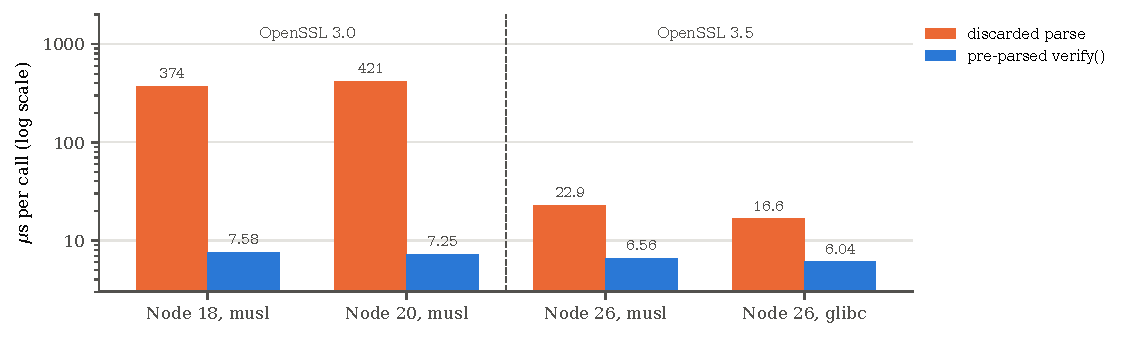
\includegraphics[width=\textwidth]{fig_runtime_matrix.pdf}
\caption{The four container rows of Table~\ref{tab:matrix} on a logarithmic
axis. The discarded parse spans \SpanProbeThrows$\times$ across images while the
pre-parsed call spans \SpanJwtPreparsed$\times$. The dashed rule marks the
OpenSSL series boundary; it is \emph{not} a controlled boundary, because the two
fast images also carry a newer engine and a different build
(Section~\ref{sec:cannot-separate}). The uncontainerised host row is omitted
because its comparison with the container rows is confounded. Generated by
\texttt{figures/make\_figures.py}~\cite{artifact2026}.}
\label{fig:matrix}
\end{figure*}

\subsection{Engine major version does not distinguish the two slow runtimes}

Node \NodeEighteenNodeMajor{} and Node \NodeTwentyNodeMajor{} ship V8
\NodeEighteenVeight{} and \NodeTwentyVeight{} --- different major versions of the
engine --- and share the OpenSSL \NodeEighteenOpensslSeries{} series. Both pay of
order \NodeEighteenProbeThrows--\NodeTwentyProbeThrows~$\mu$s. Node
\NodeTwentySixMuslNodeMajor{} ships OpenSSL \NodeTwentySixMuslOpensslSeries{} and
pays \NodeTwentySixMuslProbeThrows~$\mu$s on the same libc. Within the OpenSSL
\NodeEighteenOpensslSeries{} series, then, changing the engine's major version
does not move the quantity; had Node \NodeTwentyNodeMajor{} been fast, the
attribution would have been to the engine.

\subsection{What this design cannot separate}\label{sec:cannot-separate}

That argument establishes a negative within one OpenSSL series. It does not
establish the positive attribution for the change between series, and we state
the limitation rather than leaving it implicit.

The fast rows are Node \NodeTwentySixMuslNodeMajor. They carry OpenSSL
\NodeTwentySixMuslOpensslSeries{} \emph{and} V8 \NodeTwentySixMuslVeight{}
\emph{and} every other change in that build. OpenSSL version is therefore
perfectly confounded with engine version and with build configuration across the
\NodeEighteenOpensslSeries--\NodeTwentySixMuslOpensslSeries{} boundary. Nothing
in this matrix can separate them. The absence of variation between V8
\NodeEighteenVeight{} and V8 \NodeTwentyVeight{} does not license the inference
that V8 \NodeTwentySixMuslVeight{} is also irrelevant; that is a different
comparison, and we did not make it.

What the matrix supports is the following, and no more: the magnitude co-varies
with the bundled OpenSSL version across four images; the two slow images differ
in engine major version and do not differ in magnitude; and the two libc variants
of one image differ by less than the difference between series. Separating
OpenSSL from the engine requires a crossed design --- a single Node version
linked against both OpenSSL series, or the parse measured outside Node entirely
--- which we did not run. We therefore write \emph{co-varies with} throughout,
including in the abstract and the conclusion, and we draw no causal conclusion
about OpenSSL from this data.

The engineering evidence cited in Section~\ref{sec:gaps} proposes a mechanism for
such a regression. We do not adopt it, for the reason given there: it is not
peer-reviewed and was not produced under a protocol we can assess.

\subsection{The effect is confined to key parsing}

Across the four container rows, pre-parsed validation spans
\SpanJwtPreparsed$\times$, the HMAC primitive \SpanHmacString$\times$ and
structural decode \SpanDecodeOnly$\times$. The discarded parse spans
\SpanProbeThrows$\times$. The successful parse moves with it
(\SpanProbeSucceeds$\times$), so this is the cost of key parsing in general
rather than anything peculiar to the failure path. The failure is simply the case
in which an application pays that cost on every request for a result it discards.

\subsection{What this design does not isolate}

A reader may notice that the uncontainerised host row is of the same order as the
Node \NodeTwentySixGlibcNodeMajor{} container row. That comparison is confounded
and we draw no conclusion about containerisation from it: the host runs a
different operating system from the containers, so operating system, C library
and Node build all change alongside the container boundary. Isolating
containerisation would require a Linux-native baseline, which we did not obtain.
The claims above concern only the four container rows, among which
containerisation is constant.

%% ============================================================================
\section{RQ3: Deployment and prevalence}\label{sec:rq3}

\subsection{In-situ cost across arrival rates}\label{sec:insitu}

The deployed service was driven at seven arrival rates, each measured by the
paired-scrape difference of Section~\ref{sec:insitu-method}, with the whole sweep
run ascending and then descending on one process. Table~\ref{tab:insitu} reports
the range across the two passes at each rate for the configuration the service
deploys, a string secret, and Figure~\ref{fig:insitu} plots it.

\begin{table}[t]
\caption{In-situ validation cost with a string secret, by arrival rate. The two
columns are the ascending and the descending pass over the same seven rates on
one process; each is a single window, and the pair is two observations rather
than an interval. Host load average during each window is committed with the
measurement.}
\label{tab:insitu}
\begin{tabular}{@{}lrr@{}}
\toprule
Arrival rate & \multicolumn{2}{c}{Mean per call ($\mu$s)} \\
(requests/s) & ascending & descending \\
\midrule
\InsituRateA & \InsituStringAscA & \InsituStringDescA \\
\InsituRateB & \InsituStringAscB & \InsituStringDescB \\
\InsituRateC & \InsituStringAscC & \InsituStringDescC \\
\InsituRateD & \InsituStringAscD & \InsituStringDescD \\
\InsituRateE & \InsituStringAscE & \InsituStringDescE \\
\InsituRateF & \InsituStringAscF & \InsituStringDescF \\
\InsituRateG & \InsituStringAscG & \InsituStringDescG \\
\bottomrule
\end{tabular}
\end{table}

\begin{figure}[t]
\centering
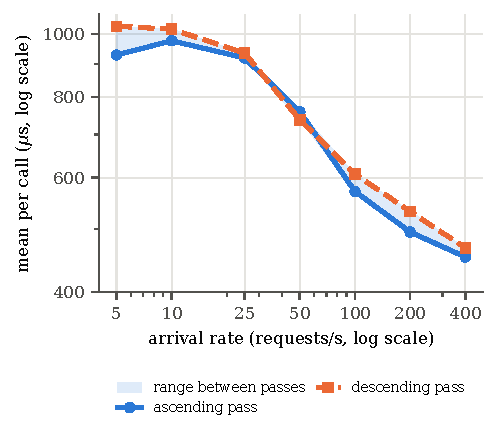
\includegraphics[width=\columnwidth]{fig_insitu_rate.pdf}
\caption{In-situ validation cost against arrival rate, string secret. The two
passes are drawn separately rather than averaged: Section~\ref{sec:drift} reports
that they differ systematically, and averaging would conceal that. The shaded
band is the range between the passes, which is two observations rather than an
interval. Generated by
\texttt{figures/make\_figures.py}~\cite{artifact2026}.}
\label{fig:insitu}
\end{figure}

One observation follows, and it is the one this section claims: the cost is
present in deployment and is far larger than the isolated host figure of
Table~\ref{tab:host}, consistent with Section~\ref{sec:rq2} in that the deployed
runtime is the one carrying the older OpenSSL.

Two things visible in Table~\ref{tab:insitu} are \emph{not} claimed, and we set
them out explicitly.

\paragraph{The magnitude is not reconciled with the microbenchmark.} The deployed
runtime's discarded parse costs \NodeEighteenProbeThrows~$\mu$s
(Table~\ref{tab:matrix}), and the remainder of the validation path is of order
\NodeEighteenJwtPreparsed~$\mu$s, giving an expected total near
\InsituPredictedFromMatrix~$\mu$s. The observed figures are
\InsituObservedLo--\InsituObservedHi~$\mu$s. Contention inflates a duration
rather than deflating it, so these are upper bounds and are not inconsistent
with the microbenchmark; but a gap of roughly
\InsituUnaccountedLo--\InsituUnaccountedHi~$\mu$s is unaccounted for, and we
report it as unaccounted rather than attributing it. It was not decomposed.

\paragraph{The decline with arrival rate is not interpreted.} Cost falls
monotonically from \InsituStringAscA~$\mu$s at \InsituRateA~requests/s to
\InsituStringAscG~$\mu$s at \InsituRateG~requests/s. This is the opposite of what
contention alone would produce, and several mechanisms unrelated to validation
would produce it --- a fixed per-window overhead amortising over more calls,
processor frequency scaling and idle-state exit latency at low rates, cache and
branch-predictor residency, or continued tier-up in the engine. We did not run
the conditions that would distinguish them. We therefore report the numbers and
do not claim that validation cost depends on arrival rate; establishing that
would require varying window duration at fixed rate, pinning the frequency
governor, and extending warmup at low rates, none of which we did.

\subsection{The two passes differ systematically}\label{sec:drift}

Sweeping up and then down is not only replication; it detects warm-up, thermal
and hysteresis effects. If the difference between passes were noise, its sign
would alternate across rate points. It does not. In the string-secret sweep the
descending pass is slower at \InsituStringSameSign{} of \InsituStringPoints{}
rate points; in the pre-parsed sweep the descending pass is \emph{faster} at
\InsituPreparsedSameSign{} of \InsituPreparsedPoints. A consistent sign across
seven points is not what noise produces.

This has a direct consequence for how the ranges in Table~\ref{tab:insitu} should
be read. A systematic component means the two passes are not independent samples
of a common value, so the range between them understates uncertainty further than
a range of two already does. We therefore report ranges and draw no inference that
depends on their width. It is also a methodological finding in its own right: a
single-direction sweep would have produced a curve carrying a consistent bias with
no way to detect it.

\subsection{Host load, not the condition, drives the outliers}\label{sec:load}

Agreement between passes varies considerably across windows. We distinguish
\emph{relative} disagreement, the gap between passes as a fraction of their mean,
from \emph{absolute} disagreement, the gap in microseconds; the two behave
differently and the distinction carries this subsection.

The widest relative disagreement in the dataset and the tightest occur at the same
arrival rate in different sweeps. The wide one is the highest-load window in its
own sweep on the descending pass, though not on the ascending pass, whose maximum
load falls at a different rate. The tight one, at the same arrival rate in another
sweep, sits at a lower load on both passes and its two passes agree to within
\InsituTightestAgreement~$\mu$s. Relative disagreement therefore does not track
the condition under measurement.

We considered two alternative explanations for the relative asymmetry and reject
both. A small-mean effect would require absolute disagreement to be roughly
constant, so that its relative size grew only as means shrank; absolute
disagreement instead varies over three orders of magnitude and is largest where
the means are largest, which is the opposite pattern. A measurement floor would
require the affected values to sit at the instrument's resolution; they do not,
and in any case the means reported here are computed from the histogram's sum and
count rather than from its buckets, so bucket resolution cannot bound them.

The operative consequence is that in-situ figures are reported with the host load
recorded during their window, and comparisons between windows at different loads
are not treated as comparisons between conditions.

\ifabdata
\subsection{Corroboration: the cost belongs to the validation
call}\label{sec:abcorroboration}
%% If an arm records PROCESS CPU TIME rather than wall clock, use this title
%% instead and swap in the commented paragraph below:
%% \subsection{Corroboration: the cost is real processor time}

An in-situ figure of this magnitude has two readings. Either it is work the
service performs, or it is an artefact of the surrounding measurement ---
ambient handler cost that would be there without validation, or a property of
the instrument rather than of the code. We separate them with an A/B of the same
service at one arrival rate, with validation enabled in one window and disabled
in the next under otherwise identical conditions. Table~\ref{tab:ab} reports it.

\begin{table}[t]
\caption{Validation enabled against validation disabled, run
\texttt{\ABRunId}, at \ABRate~requests/s over \ABWindowSeconds~s per window.
The means time \ABQuantity, computed as the difference of the histogram's
\texttt{\_sum} divided by the difference of its \texttt{\_count}, as in
Section~\ref{sec:insitu-method}. \emph{Two caveats govern how this table may be
read.} First, the load figure is a single \texttt{uptime} sample taken at window
start --- the same quantity and capture path as the per-window load recorded
with the rate sweeps --- and not a mean over the window; no within-window load
series exists for these two runs. Second, the difference is a difference of two
window means, not the median of per-round paired differences used everywhere
else in this paper (Section~\ref{sec:unit}), because the two arms are separate
windows and cannot be paired. It is the only quantity in the paper of that kind,
and no other result depends on it.}
\label{tab:ab}
\small\setlength{\tabcolsep}{4pt}
\begin{tabular}{@{}lrrr@{}}
\toprule
            & Mean per call & Calls & Load at \\
Arm         & ($\mu$s)      &       & window start \\
\midrule
validation enabled  & \ABEnabledMean  & \ABEnabledCalls  & \ABEnabledLoad  \\
validation disabled & \ABDisabledMean & \ABDisabledCalls & \ABDisabledLoad \\
\midrule
difference          & \ABDelta        &                  &                 \\
\bottomrule
\end{tabular}
\end{table}

Removing validation removes \ABDelta~$\mu$s per call, \ABDeltaPct\% of the
enabled mean. The arrival rate, the request path and the rest of the handler are
unchanged between the arms; only the validation call is withdrawn. The in-situ
figure is therefore attributable to that call rather than to ambient handler
cost or to the instrument, which is what this table is for.

Whether the time is spent executing or spent descheduled inside the call is a
further question, and a wall-clock difference does not answer it. Three
observations together do. The isolated microbenchmark of Section~\ref{sec:rq1}
measures the same operation in a single process with no concurrent load at all
and finds it dominated by the same component. The sampling profiler of
Section~\ref{sec:rq1} attributes a median \ProfHostPct\% of \emph{self} time to
that frame, and self time is time on processor. And the A/B above shows the cost
survives into deployment and belongs to the call. The microbenchmark and the
profiler establish that the work is processor time; the A/B establishes that the
deployed figure is the same work and not something else.

%% CPU-TIME alternative. Use INSTEAD of the two paragraphs above, with the
%% original subsection title, ONLY if an arm records process CPU time. Replace
%% the bracketed phrase with what was actually recorded.
%%
%% Removing validation removes \ABDelta~$\mu$s per call, \ABDeltaPct\% of the
%% enabled mean. Because the means are computed from [process CPU time rather
%% than wall clock], the difference is processor time and not time the request
%% spent queued or descheduled: a request that waits accrues no CPU. The arrival
%% rate, the request path and the rest of the handler are unchanged between the
%% arms; only the validation call is withdrawn. This is the deployment-side
%% counterpart of the profiler attribution in Section~\ref{sec:rq1}, which
%% assigns a median \ProfHostPct\% of self time to the same frame in isolation.

That is the whole of what this table establishes, and we are explicit about what
it does not. It does not reconcile the in-situ magnitude with the microbenchmark:
Section~\ref{sec:insitu} reports a gap of roughly
\InsituUnaccountedLo--\InsituUnaccountedHi~$\mu$s between the observed means and
the sum of the components measured on the deployed runtime, and one A/B at one
rate does not decompose it. It does not bound the contribution of host load,
because the load figures are window-start snapshots rather than means. And two
windows are two observations: the difference carries no interval, and we compute
none from it.

\else

\subsection{Corroboration: the cost is not an artefact of the
instrument}\label{sec:abcorroboration}

An in-situ figure of this magnitude has two readings. Either it is work the
service performs, or it is an artefact of the surrounding measurement --- ambient
handler cost that would be there without validation, or a property of the
instrument rather than of the code. The second is excluded by an A/B of the same
service at one arrival rate, with validation enabled in one window and disabled
in the next under otherwise identical conditions; the two runs are committed with
the rest of the measurements in the replication package~\cite{artifact2026}.
Withdrawing the validation call, with the arrival rate, the request path and the
remainder of the handler unchanged, removes the great majority of the per-call
cost, which locates it in that call.

Whether the time is spent executing or spent descheduled inside the call is a
further question that this comparison does not answer. Two instruments do. The
isolated microbenchmark of Section~\ref{sec:rq1} measures the same operation in a
single process with no concurrent load at all and finds it dominated by the same
component, and the sampling profiler of Section~\ref{sec:rq1} attributes a median
\ProfHostPct\% of \emph{self} time to that frame, self time being time on
processor.

\fi

\subsection{How common is the avoiding pattern, in our
sample?}\label{sec:prevalence}

Three instruments, three frames, reported separately as Section~\ref{sec:frames}
requires. All counts were captured on \PopCapturedAt. None of the figures below
is a population proportion.

\paragraph{Population co-occurrence.} Of \PopJsRequireFiles{} public JavaScript
files importing the library through \texttt{require},
\PopJsRequireFilesWithApi{} also mention the pre-parsing interface; for
JavaScript through \texttt{import} the figures are \PopJsImportFiles{} and
\PopJsImportFilesWithApi; for TypeScript through \texttt{require},
\PopTsRequireFiles{} and \PopTsRequireFilesWithApi; and for TypeScript through
\texttt{import}, \PopTsImportFiles{} and \PopTsImportFilesWithApi. Cells are not
pooled into a rate: a file using both import forms would be counted twice, so
their sum \PopSumFiles{} is an upper bound on the union and the largest cell
\PopLargestCellFiles{} a lower bound. No cell exceeds \PopWorstCellPct\% of files
mentioning the interface. These are search-engine estimates of file counts over
public repositories only, they measure co-occurrence rather than use, and the
denominators are returned \emph{rounded} --- each is an exact multiple of $1024$
--- so they should be read as magnitudes rather than as counts established file
by file.

\paragraph{Classified call sites.} Of \SampleCallSites{} call sites classified
across \SampleRepos{} distinct repositories in our sample,
\SampleSitesPreparsed{} pass a pre-parsed key. Environment variables account for
\SampleEnvString{} of those call sites, untraced identifiers and member
expressions \SampleUnknown{}, string literals \SampleStringLiteral{}, file
contents \SampleFileContents{} and buffers \SampleBuffer. No file in this corpus
contains the pre-parsing interface at all, in any spelling, so the zero reflects
the pattern's absence from the sample rather than a classifier that cannot see
it. Incidentally, \SampleNoAlgorithms{} of \SampleCallSites{} call sites
(\SampleNoAlgorithmsPct\%) pass no algorithm restriction, which
Section~\ref{sec:fix} returns to.

An earlier version of the classifier recognised only the conventional
\texttt{jwt.verify()} spelling, which filtered the corpus toward one import
idiom. It was re-run over the previously unclassified residue with a matcher that
resolves the local binding of the import --- covering arbitrary aliases,
namespace imports, destructured and renamed imports, and direct calls on the
require expression. That recovered \SampleRematchAdded{} further call sites,
included in the totals above, of which \RematchSitesPreparsed{} pass a pre-parsed
key.

\paragraph{Targeted counter-search.} A sample can only show a pattern is rare if
it could have found it. Every file co-occurring the library with the pre-parsing
interface was therefore fetched: \CounterFilesFetched{} files, of which
\CounterWithVerify{} contain a validation call, spanning
\CounterReposWithVerify{} distinct repositories. An automated pass flagged
\AdjudicatedTotal{} call sites as passing a pre-parsed key and all were then read
by hand: \AdjudicatedFalsePositive{} are false positives --- projects defining
their own helper function of the same name, one of which returns a string ---
\AdjudicatedUnresolved{} could not be resolved within its file, and
\AdjudicatedGenuine{} are genuine, across \AdjudicatedGenuineProjects{} distinct
projects.

\paragraph{The rate, with its denominator.} Among the \CounterReposWithVerify{}
repositories that both reference the pre-parsing interface and call the
validator, \AdjudicatedGenuineProjects{} use it: \AdjudicatedGenuinePct\%. That
denominator is the most favourable available, since those projects demonstrably
know the interface exists, and it is not the population. Within this frame the
pattern is rare rather than absent, and it is rare even among projects already
aware of it. We do not extrapolate beyond the frame.

%% ============================================================================
\section{A fix, and a constraint on it}\label{sec:fix}

The fix is to dispatch on the token's declared algorithm before attempting the
asymmetric parse, so that an HMAC token with an ordinary string secret is
resolved directly. Applied, this takes the call from \HostJwtString~$\mu$s to
\HostJwtStringSafe~$\mu$s, a factor of \HostSafePatchRatio, and to within
\HostSafePatchResidual~$\mu$s of supplying a pre-parsed key, with no change in
calling code. That residual is the median of the per-round paired differences,
not the difference of the two medians; the two are not identical and the former
is reported throughout.

We tested it against the library's own suite rather than only against assertions
of our own. Cloned at \LibraryTag, the patch applies cleanly and the suite is
unchanged: \SuiteStockPassing{} passing and \SuiteStockFailing{} failing
unpatched, \SuitePatchedPassing{} and \SuitePatchedFailing{} patched.

These figures are from the host. The practical benefit is largest where the
discarded parse is largest --- of order \NodeEighteenProbeThrows~$\mu$s on the
runtime the service actually deploys (Table~\ref{tab:matrix}) --- and we did not
measure the patched library on the container runtimes. The reported factor of
\HostSafePatchRatio{} is therefore a lower bound on the improvement available in
the deployed environment, and we state it as a host result rather than as a
general one.

\paragraph{The constraint, which is the more important half.} The discarded
attempt is not purely wasteful. The \emph{success} of that parse on asymmetric
key material is what produces a key object whose type a later check depends on,
and that check is what prevents symmetric and asymmetric material from being
interchanged~\cite{rfc8725}. A change that dispatches on the declared algorithm
while relaxing which key material may take the fast path alters which inputs
reach that check.

The fix must therefore be narrow: the fast path is restricted to string secrets
that cannot be asymmetric key material, so anything that might be resolves
exactly as it does today. Removing that material restriction --- the form of the
optimisation we argue against --- produces \SuiteNaiveFailing{} failures in the
library's own suite, both in its key-confusion tests
(\NaiveFailingTests).

\paragraph{A reduction of our own contribution.} We had written a regression test
for this property and intended to offer it upstream. Running the library's
existing suite showed that it already constrains the change: a contributor
proposing the unrestricted optimisation would be caught by tests they are
required to run. We therefore withdraw that contribution. What remains is
narrower and, we think, still worth stating: the cost documented in
Section~\ref{sec:rq1} cannot be removed by the obvious route, and the reason is a
property the maintainers already test for but which is not evident from the code
being changed.

The independent defence against this class of confusion is for the caller to
restrict permitted algorithms~\cite{rfc8725}, and \SampleNoAlgorithmsPct\% of the
call sites surveyed in Section~\ref{sec:prevalence} do not.

%% ============================================================================
\section{Implications for practice}\label{sec:implications}

\paragraph{Pre-parse key material once, at startup.} On the host this removes
\HostStringPenalty~$\mu$s per validation
[\HostStringPenaltyCiLo, \HostStringPenaltyCiHi]; on the runtime the service
actually deploys, where the discarded parse costs
\NodeEighteenProbeThrows~$\mu$s, it removes far more. It requires no
architectural change, no new component and no movement of a trust boundary.

\paragraph{Treat the base image as part of the measurement.} The same code, the
same library and the same architecture differ by \SpanProbeThrows$\times$ on this
path across the container images measured, because they pin different OpenSSL
versions. A performance figure quoted without the base image it was obtained on
is not reproducible, and a regression appearing after a base-image bump may have
nothing to do with the application. This holds whether or not the OpenSSL version
is the cause, which Section~\ref{sec:cannot-separate} states we cannot establish;
it is enough that the image changes the number.

\paragraph{Pin the algorithm.} Independently of anything here, callers should
restrict permitted algorithms~\cite{rfc8725}. Most of the call sites we surveyed
do not, which leaves them relying entirely on library-internal key typing for a
property they could assert directly in one argument.

\subsection{Relocation is not the first remedy}\label{sec:offload}

Because a cost believed to be cryptographic invites relocation, we implemented
that relocation and report what it does. This subsection rests on source
inspection and a manual observation; it carries no measured result, and we set
out below why we report none.

Applying a mesh \texttt{RequestAuthentication} policy causes the sidecar to
validate the token before proxying. It does not cause the application to stop
validating: verification is \emph{duplicated}, not relocated, and no work leaves
the event loop. Making relocation effective therefore requires the application to
trust something the sidecar tells it. In our implementation the handler reads a
sidecar-populated claims header and, when it is present, returns the protected
payload without verifying anything --- the branch is a single conditional in
\texttt{service-a/index.js} in the replication package~\cite{artifact2026}.

Trusting an identity header injected by an upstream proxy, without stripping any
client-supplied copy at the trust boundary and without a fail-closed path when
the policy is not applied, is a known deployment anti-pattern rather than a novel
finding, and we report it as such. In our implementation the sidecar overwrites
the header only while a policy is applied; in any other state nothing sanitises
it. With the guard filter applied, a request carrying a forged claims header and
no credential is refused. With the guard removed, the same request returns the
protected payload. We reproduced this sequence manually --- refused, served,
refused --- and it is consistent with the note recorded alongside the affected
runs in the replication package. The remedy is an always-applied filter that
strips any client-supplied copy of the header on entry to the pod, before any
validation filter runs, matched on the connection manager rather than on the
validation filter, because in the state that needs protection no validation
filter exists.

\paragraph{Why we report no measured result.} We wrote an automated probe to turn
the observation into a table and it does not produce a trustworthy one. The mesh
applies a configuration change asynchronously, on a timescale comparable to the
probe interval, so whether a probe observes the guarded or the unguarded
behaviour depends on whether the proxy had converged when the request fired. Two
runs of the same script produced contradicting values for the same configuration.
Rather than report the run that agreed with our expectation, we report none: the
script's own negative control declared both runs inconclusive, and we retain it
in the replication package with that limitation recorded. Making this measurable
requires gating each probe on \emph{observed} configuration convergence ---
polling until repeated identical responses --- rather than on a fixed delay. We
have not implemented that, and until it is done this subsection should be read as
a mechanism argument supported by an observation, not as a measurement.

The narrow point that survives is the one this paper's measurements support: the
cost documented in Section~\ref{sec:rq1} is largely avoidable in place, so an
architectural remedy that also moves a trust boundary should not be the first
thing reached for.

%% ============================================================================
\section{Threats to validity}\label{sec:threats}

\paragraph{One architecture.} Every measurement comes from a single ARM64 host
and its container runtimes under one engine. We have not verified any of this on
x86\_64. The mechanism is a property of a library's API contract --- an
asymmetric parse attempted before a symmetric one, with the failure discarded ---
and of the cost of key parsing in a particular OpenSSL series, and neither is a
property of an instruction set. But an expectation is not a measurement, and the
magnitude in particular depends on how OpenSSL's key parsing performs on a given
platform, which is exactly the kind of quantity that varies with architecture. No
claim here should be read as holding beyond ARM64.

\paragraph{OpenSSL and engine version cannot be separated.} As
Section~\ref{sec:cannot-separate} states, the fast rows carry a newer OpenSSL, a
newer engine and a different build simultaneously. The matrix establishes that
the magnitude co-varies with the OpenSSL series and that engine major version
does not distinguish the two slow runtimes; it does not establish that OpenSSL is
the cause of the difference between series. A crossed design would settle it and
we did not run one.

\paragraph{The \HostProbeThrows~$\mu$s is not decomposed.} The dominant component
is a discarded parse attempt together with the exception that terminates it. We
report the pair. Section~\ref{sec:granularity} gives the one bound our data
supports and states why we cannot do better without an instrument inside OpenSSL.

\paragraph{One host figure cannot be version-attributed.} The host decomposition
of Section~\ref{sec:rq1} predates the per-measurement OpenSSL field, and the
host's OpenSSL has since moved by a patch release, so the version that produced
those figures is known by run timestamp rather than from the measurement record.
Table~\ref{tab:matrix} therefore leaves the host OpenSSL cell unrecorded rather
than filling it with a version captured later. Since Section~\ref{sec:rq2} shows
this quantity varies \SpanProbeThrows$\times$ with the runtime, this is a
material limitation on the headline figure and not a bookkeeping detail: the
\HostProbeThrows~$\mu$s is attributable to the host as configured at that time
and to nothing more specific. The container rows, which carry the attribution of
Section~\ref{sec:rq2}, each record their own.

\paragraph{Ranges of two, with a systematic component.} The in-situ dispersion is
the range across an ascending and a descending pass. It is not a confidence
interval, and Section~\ref{sec:drift} shows the two passes differ systematically
rather than randomly, so they are not independent samples of a common value and
the range understates uncertainty further. No inference in this paper depends on
the width of those ranges.

\paragraph{One in-situ process, two passes.} The whole deployment result rests on
one process sweeping seven rates twice. That is sufficient for the claim made ---
the cost is present in deployment and of this order --- and insufficient for any
claim about the shape of the cost-versus-rate relation, which
Section~\ref{sec:insitu} accordingly does not make.

\paragraph{The in-situ magnitude is unreconciled.} The observed
\InsituObservedLo--\InsituObservedHi~$\mu$s exceeds the sum of the measured
components on the deployed runtime by a margin we did not decompose, and the
decline with arrival rate has several candidate explanations unrelated to
validation that we did not test. Section~\ref{sec:insitu} states both as
unaccounted rather than interpreting them.

\paragraph{Sampling frames are not interchangeable.} The three prevalence
instruments of Section~\ref{sec:frames} have different units and different
selection mechanisms, and none supports a population proportion. The
co-occurrence counts measure two strings appearing in one file, with a
false-positive rate established at \AdjudicatedFalsePositive{} of
\AdjudicatedTotal{} on hand inspection. The classified sample has unknown
inclusion probabilities, a limitation of repository search noted more generally
by Kalliamvakou et al.~\cite{kalliamvakou2014promises}. The counter-search is
selected on the outcome.

\paragraph{The matcher's coverage.} Call sites are found by resolving the local
binding of the import, which covers aliases, namespace imports, destructured and
renamed imports and direct calls on the require expression. It does not resolve
bindings across files, so a project that constructs a pre-parsed key in one file
and validates in another is invisible to this analysis. This is the strongest
threat to Section~\ref{sec:prevalence}; within-file tracing found no such case,
which is weak evidence against it.

\paragraph{Host load, and the confound that motivated recording it.} A
throughput curve measured on a host shared with its own load generator moves with
unrelated activity on that host, as Section~\ref{sec:hoststate} describes, which
is why no capacity claim appears in this paper. Every in-situ window here carries
the load average observed during it, and Section~\ref{sec:load} shows that window-to-window
agreement tracks that load rather than the condition. Contention inflates a
duration rather than deflating it, so in-situ figures are upper bounds; but
comparisons between windows at different loads are not comparisons between
conditions, and we do not treat them as such.

\ifabdata
\paragraph{The A/B windows carry a load snapshot, not a load series.} Every
figure in Table~\ref{tab:ab} comes from two windows whose host load is known only
at the instant each began. Section~\ref{sec:load} shows that window-to-window
agreement in the rate sweeps tracks load rather than the condition under
measurement, so a load excursion inside either A/B window would be invisible
here. Contention inflates a duration rather than deflating it and the enabled arm
is the slower one, so an unobserved excursion in that window would inflate the
difference rather than manufacture it: the direction of the conclusion is safe,
its magnitude is not. Attaching the per-second sampler used elsewhere in the
instrumentation to a re-run of both arms would remove this limitation; we did
not. The two arms are also separate windows rather than interleaved rounds, so
the design is weaker on this one comparison than the protocol of
Section~\ref{sec:unit} requires elsewhere.
\fi

\paragraph{Token caching is not in the comparison.} A service that caches
verified tokens pays this cost once per token rather than once per request. We
did not measure such a configuration, so the per-request figures here do not
describe a caching deployment.

\paragraph{One rater.} The \AdjudicatedTotal{} automatically flagged call sites
were read and classified by the first author, and the authors are not
disinterested: the paper's claim is stronger the more of them are false
positives, and \AdjudicatedFalsePositive{} were classified that way. There was no
second rater and no inter-rater agreement to report. The per-case verdicts, the
evidence for each and the hashes of the files they were read from are published
so the adjudication can be repeated, which is weaker than having repeated it.

\paragraph{One library at one version.} The mechanism is specific to one
JavaScript implementation at one release. Whether other implementations or other
language ecosystems attempt key resolution in the same order is unmeasured, and
the paper's framing --- that cryptographic cost is over-attributed --- is
therefore demonstrated for one library rather than established as a class of
defect.

%% ============================================================================
\section{Conclusion}\label{sec:conclusion}

The per-request cost of token validation in this library is real, is worth
attending to, and is not the signature: the primitive is \HostHmacString~$\mu$s
of a \HostJwtString~$\mu$s call. It is not key conversion either, which costs
\HostCreateSecretKey~$\mu$s. It is a parse attempted in the wrong order, whose
failure is constructed and thrown away on every request at
\HostProbeThrows~$\mu$s, \HostProbeShareOfCall\% of the call. We report that
quantity as the parse attempt together with the exception that ends it, because
we did not separate them.

Its price co-varies with the OpenSSL version a base image happens to pin, varying
\SpanProbeThrows$\times$ across runtimes while the rest of the validation path
varies by \SpanJwtPreparsed$\times$. We state that as a co-variation because the
available runtimes confound the OpenSSL series with the engine version shipped
alongside it.

The pattern that avoids the cost is rare in our sample: among
\CounterReposWithVerify{} repositories that already reference the pre-parsing
interface and call the validator, \AdjudicatedGenuineProjects{} use it. No
population proportion follows.

Two explanations that present themselves before the measurement are refuted by
it. That the dominant cost is key conversion is refuted by measuring the
conversion. That a throughput collapse under layered enforcement characterises
the service is refuted by the collapse point moving with unrelated host activity,
which is why no capacity claim appears here. Both have the same shape, and it is
the shape this paper's methodology is built to avoid: a cost attributed to the
variable under study while a second variable moves alongside it, unrecorded at
the granularity at which it could change. The bundled OpenSSL version in
Section~\ref{sec:rq2} is the same hazard caught in time --- the quantity varies
\SpanProbeThrows$\times$ with a component most measurement protocols record once
per run, if at all. The lesson is not that one should measure in deployment. It
is narrower: record the identity of the component whose behaviour is being
measured, on every measurement, at the granularity at which it can change.

%% ============================================================================
\backmatter

\bmhead{Data availability}
The data supporting the results of this study are openly available in the
archived replication package~\cite{artifact2026}, deposited on Zenodo under the
DOI given in that reference. It contains all measurements, the instrumentation,
the analysis code and the scripts that generate every numeric value and every
figure in this paper. Every number is generated from a file under the run or
survey directories; none is entered by hand. The survey corpus is third-party
source and is not redistributed; a manifest pinning every file examined by
content hash stands in for it, covering \ManifestFiles{} files across
\ManifestRepos{} repositories. Content hashes resolved for all of them; the
repository HEAD commit resolved for \ManifestHeadResolved{} of \ManifestFiles,
one repository having become unavailable between fetch and manifest. The content
hash is the authoritative pin and is complete.

\bmhead{Competing interests}
The authors declare no competing interests.

\bmhead{Funding}
\TODO{To be completed by the authors before submission.}

\bmhead{Author contributions}
\TODO{To be completed by the authors before submission. Springer requires a
statement of each author's contribution; the present authors' individual roles
are not recorded in the artifact and are not inferable from it.}

\bmhead{Ethics approval}
Not applicable. This study measures software behaviour and publicly available
source code; it involves no human participants and no personal data.

%% sn-jnl.cls selects the Springer .bst itself from the class option; the
%% `article` fallback needs a numeric style named explicitly.
\ifdefined\SNJNL\else\bibliographystyle{unsrt}\fi
\bibliography{discarded-exception}

\end{document}
